\documentclass[12pt, a4paper]{article}

\usepackage{import}
\usepackage{standalone}

\usepackage[top=4cm, right=2cm, bottom=2.7cm, left=2cm]{geometry}

\usepackage{wrapfig}
\usepackage{tabulary}
\usepackage{float}
\usepackage{pifont}
\usepackage{background}
\usepackage{tikz}


\pagestyle{empty}
\setlength{\parindent}{0pt}

\begin{document}
	\begin{minipage}{\textwidth}
		\section{Stambomen \hfill\small Bron: Bebras}
			
			Grootvader Bever heeft zijn stamboom op zijn computer opgeslagen. In deze stamboom werden de kinderen van elk familielid onder hun ouders geplaatst en er door lijnen mee verbonden. De kinderen worden van links naar rechts geplaatst in volgorde van hun geboortedatum.
			
			\begin{figure}[H]
				\centering
				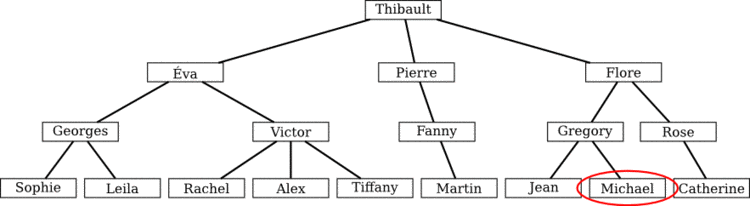
\includegraphics[width=\linewidth]{image1} 
			\end{figure}
			
			Er wordt op het computerscherm slechts \'e\'en bever tegelijk getoond. Om een ander familielid te zien, moet je een reeks opdrachten uitvoeren. Er zijn twee mogelijke opdrachten:
			\begin{itemize}
				\item De opdracht ouder toont de \textbf{ouder} van de bever die op dat moment op het scherm staat.
				\item De opdracht \textbf{kind[1]} toont het $1^{ste}$ kind (dit aan de linkerkant) van de bever die op dat moment te zien is, \textbf{kind[2]} toont het $2^{de}$ kind, enzovoort.
				In het begin staat ''Michael'' op het scherm.
			\end{itemize}
			Je voert nu de volgende opdrachten uit: \textbf{ouder, ouder, ouder, kind[1], kind[2], kind[1]}. Wat is de naam van de bever die je daarna te zien krijgt?
			
			\begin{table}[H]
				\centering 
				\begin{tabulary}{\linewidth}{|C|C|C|C|C|}
					\hline
					\textbf{A} \vspace{0.1cm}
					
					Victor
					&
					\textbf{B} \vspace{0.1cm}
					
					Georges	
					&
					\textbf{C} \vspace{0.1cm}
					
					Leila
					&
					\textbf{D} \vspace{0.1cm}
					
					Thibault
					&
					\textbf{E} \vspace{0.1cm}
					
					Tiffany
					\\ \hline
					\textbf{F} \vspace{0.1cm}
					
					Rachel	
					&
					\textbf{G} \vspace{0.1cm}
					
					Michel	
					&
					\textbf{H} \vspace{0.1cm}
					
					Martin	
					&
					\textbf{I} \vspace{0.1cm}
					
					Catherine	
					&
					\textbf{J} \vspace{0.1cm}
					
					Sophie
					\\ \hline
				\end{tabulary}
			\end{table}

	\end{minipage}
		
\end{document}